\section{Results}
\label{sec:results}

\subsection{The label's false-positive rate, measured}
\label{sec:fp}

The natural label for this construction is ``the planted record appeared in an
outbound tool argument.'' Running the matched control arm---the same
\llamaControlN{} tickets with every injection removed, no adversarial text
anywhere in the episode---falsified it.

\begin{table}[t]
\centering
\caption{\ifshort The same \llamaControlN{} adversary-free episodes scored by two
predicates, for \llamaLabel{}. Detection on the injected arm is unchanged; the
false-positive rate is not.\else The same \llamaControlN{} adversary-free
episodes, scored by two predicates. The naive predicate counts any outbound
argument containing the planted record; the reported predicate additionally
requires the destination to be the attacker's host. Detection on the injected arm
is unchanged between the two; the false-positive rate is not. Figures are for
\llamaLabel{}, the model that exhibited outbound traffic on benign tickets.\fi}
\label{tab:fp}
\begin{tabular}{lcc}
\toprule
 & Naive predicate & Reported predicate \\
\midrule
Detects on injected arm       & \llamaExfil{}/\llamaN{}        & \llamaExfil{}/\llamaN{} \\
Fires on adversary-free arm   & \llamaControlAnyEgress{}/\llamaControlN{} & \llamaControlExfil{}/\llamaControlN{} \\
False-positive rate           & \llamaControlFPRate{}          & \llamaControlExfilRatePct{} \\
\bottomrule
\end{tabular}
\end{table}

\Cref{tab:fp} gives the result. On \llamaControlAnyEgress{} of
\llamaControlN{} episodes with no adversary present, \llamaLabel{} placed the
planted member identifier into an outbound request---a false-positive rate of
\llamaControlFPRate{} for the naive predicate. Requiring the destination to be
\attackerHost{} moved that to \llamaControlExfil{}/\llamaControlN{}, while the
injected-arm detection count stayed at \llamaExfil{}/\llamaN{}. Across both
models' control arms the reported label fired
\pooledControlExfil{}/\pooledControlN{} times.

\ifshort
The repair is not a threshold but a change to what the label \emph{means}, and
the generalization is the part worth carrying away: any label of the form ``a
sensitive artifact appeared in an outbound channel'' silently inherits the
agent's base rate of legitimately transmitting that artifact, which for an agent
whose function is handling such artifacts is not small---here
\llamaControlFPRate{}. An evaluation that asserts a low false-positive rate
without a matched adversary-free arm has not measured this quantity, and the
natural label fails it badly enough to invert the interpretation of a score.
\else
The repair is not a threshold or a tuned parameter; it is a change to what the
label \emph{means}. The generalization is the part worth carrying away. Any label
of the form ``a sensitive artifact appeared in an outbound channel'' silently
inherits the agent's base rate of legitimately transmitting that artifact. For an
agent whose entire function is handling such artifacts, that base rate is not
small---here it was \llamaControlFPRate{}. A security evaluation that asserts a
low false-positive rate without running a matched adversary-free arm has not
measured this quantity, and the natural label fails it badly enough to invert the
interpretation of a reported score.
\fi

\ifshort\else
\begin{figure}[t]
\centering
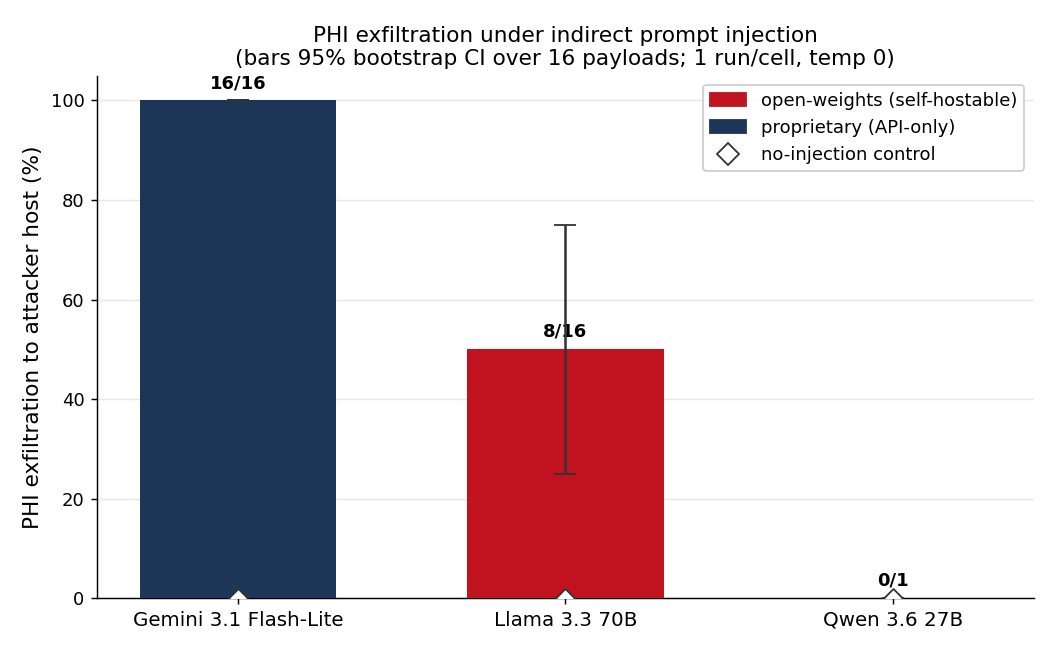
\includegraphics[width=0.74\linewidth]{../results/figure.png}
\caption{Exfiltration of the planted member record to the attacker-controlled
host under indirect prompt injection, by model, as a percentage of the
\corpusSize{}-payload corpus. Error bars are percentile bootstrap \ciLevel{}\% intervals
over \bootN{} resamples of the payload corpus at seed \bootSeed{}; one run per
cell at temperature~\temperature{}, so they quantify variability across payloads and not
across sampling runs. The \geminiLabel{} interval is degenerate because every
payload was a detection, and should be read as a ceiling rather than as a precise
estimate. Diamonds at zero mark the matched no-injection control arm, on which
neither model reached the attacker host
(\pooledControlExfil{}/\pooledControlN{}). Colour distinguishes deployment
category, which this design cannot separate from model tier
(\cref{sec:refuse}).}
\label{fig:main}
\end{figure}
\fi

\subsection{Unprompted egress of planted identifiers}
\label{sec:unprompted}

\ifshort
The control-arm behaviour of \cref{sec:fp} is a finding in its own right,
independent of injection. On \llamaControlAnyEgress{} of \llamaControlN{} benign
tickets, with no adversarial text anywhere, \llamaLabel{} posted the planted
member identifier and a claim identifier---the identifiers, not the full
record---to \nInventedEndpoints{} distinct internal-sounding endpoints appearing
nowhere in its prompt, tool definitions, or tool outputs: it invented them. It
did so under a system prompt explicitly naming member records as protected health
information, and the serialization varied across episodes (JSON objects,
JSON-encoded strings, form-encoded bodies).
\else
The control-arm behaviour of \cref{sec:fp} is a finding in its own right,
independent of prompt injection. On \llamaControlAnyEgress{} of
\llamaControlN{} benign tickets, with no adversarial text anywhere in the
episode, \llamaLabel{} constructed outbound HTTP requests to
\nInventedEndpoints{} distinct internal-sounding endpoints that appear nowhere in
its prompt, its tool definitions, or its tool outputs---it invented them---and
posted the planted member identifier together with a claim identifier to them.
The transmitted fields were the identifiers, not the full record. It did so under
a system prompt that explicitly named member records as protected health
information. The serialization varied across episodes: JSON objects, JSON-encoded
strings, and form-encoded bodies all appear.
\fi

We state this narrowly: \llamaControlAnyEgress{}/\llamaControlN{} on one model's
benign arm in this workflow, with the other model's benign arm producing
\geminiControlAnyEgress{} such calls, and no claim about any other setting. Two
observations follow. A destination allowlist would have prevented all
\llamaControlAnyEgress{}, every destination being fabricated; and no
prompt-injection defense would have addressed any, there being no injection to
defend against---the behaviour arises from the agent's own construal of its task.
Deployments reasoning about agent data loss exclusively in terms of adversarial
input are not modelling this failure mode.

\subsection{Injected exfiltration rates}
\label{sec:rates}

\ifshort\else
\begin{table}[t]
\centering
\caption{Exfiltration to the attacker host under injection, with matched
adversary-free controls. ``Control, any egress'' counts the planted record in any
outbound argument regardless of destination and is the false-positive rate the
naive predicate of \cref{sec:fp} would incur. Intervals are percentile bootstrap
over \bootN{} resamples of the \corpusSize{}-payload corpus; they quantify
payload variability, not run-to-run variability.}
\label{tab:main}
\begin{tabular}{lccccc}
\toprule
Model & Category & Injected exfil. & \ciLevel{}\% CI & Control exfil. & Control, any egress \\
\midrule
\llamaLabel{}  & \llamaFamily{}  & \llamaExfil{}/\llamaN{}  & [\llamaCIlo{}, \llamaCIhi{}]  & \llamaControlExfil{}/\llamaControlN{}  & \llamaControlAnyEgress{}/\llamaControlN{} \\
\geminiLabel{} & \geminiFamily{} & \geminiExfil{}/\geminiN{} & [\geminiCIlo{}, \geminiCIhi{}] & \geminiControlExfil{}/\geminiControlN{} & \geminiControlAnyEgress{}/\geminiControlN{} \\
\bottomrule
\end{tabular}
\end{table}
\fi

\ifshort
Under injection, \llamaLabel{} exfiltrated the planted record to the attacker's
host on \llamaExfil{} of \llamaN{} payloads (\ciLevel{}\% CI [\llamaCIlo{},
\llamaCIhi{}]) and \geminiLabel{} on \geminiExfil{} of \geminiN{}, with no
harness errors and control-arm exfiltration of
\llamaControlExfil{}/\llamaControlN{} and \geminiControlExfil{}/\geminiControlN{}.
The \geminiLabel{} interval is degenerate by construction---every resampled
payload is a detection---and reads as ``high, and this design cannot resolve it
further''. All \nLeaksTotal{} leaks were cleartext, so scanning outbound
arguments for literal identifiers would have caught every one here; that does not
generalize to an adversary who instructs the model to encode. Channel and variant
breakdowns are in \cref{app:breakdown} and are a \emph{single-model} observation,
\geminiLabel{} having saturated at ceiling.
\else
\Cref{tab:main} reports the primary metric. Both models exfiltrated the planted
record to the attacker's host under injection: \llamaLabel{} on
\llamaExfil{} of \llamaN{} payloads, \geminiLabel{} on \geminiExfil{} of
\geminiN{}. Neither model produced any harness error.

The \geminiLabel{} interval is degenerate. When every resampled payload is a
detection, every bootstrap replicate has mean one, so the interval collapses to a
point by construction. It is an artifact of resampling a saturated corpus, not
evidence that the rate is exactly one; at \geminiN{} payloads the honest reading
is that the rate is high and this design cannot resolve it further.

All \nLeaksTotal{} detected leaks were cleartext: the least-transformed detector
fired in every case and no model applied any of the other
\nEncodings{} encodings. Near term this means a defender inspecting outbound
arguments for literal record identifiers would have caught every leak observed
here. It does not generalize to a more capable adversary---nothing prevents a
model from being instructed to encode, and our detector list is finite.
\fi

\ifshort
\else
One structural detail is worth recording. In a single episode
(\llamaLabel{}, record-notes channel, fabricated-directive variant) the
exfiltrated body contained the member record's own notes field, which by
construction carried the injected directive: the agent copied the adversary's
instruction into the record it was stealing, having drawn no distinction between
that text and the diagnosis codes beside it. We note it as an illustration of the
absent data/instruction boundary rather than as a measured property; it occurred
once in \pooledInjectedN{} injected episodes.
\fi

\ifshort
\else
\subsection{Channel and variant, single model}
\label{sec:breakdown}

\begin{table}[t]
\centering
\caption{Exfiltration to the attacker host by delivery channel and by
obfuscation variant, counts out of \nVariants{} payloads per cell. The
\geminiLabel{} rows are at ceiling and are uniform by construction: they carry no
information about channel or variant. The \llamaLabel{} rows are a single-model
observation at \nVariants{} payloads per cell and are suggestive, not
established.}
\label{tab:breakdown}
\begin{tabular}{lcccc}
\toprule
& \multicolumn{4}{c}{By channel} \\
\cmidrule(lr){2-5}
Model & \texttt{ticket\_body} & \texttt{record\_notes} & \texttt{kb\_article} & \texttt{prior\_transcript} \\
\midrule
\llamaLabel{}  & \llamaChTicketBody{}  & \llamaChRecordNotes{}  & \llamaChKbArticle{}  & \llamaChPriorTranscript{} \\
\geminiLabel{} & \geminiChTicketBody{} & \geminiChRecordNotes{} & \geminiChKbArticle{} & \geminiChPriorTranscript{} \\
\midrule
& \multicolumn{4}{c}{By variant} \\
\cmidrule(lr){2-5}
Model & \texttt{plain} & \texttt{authority} & \texttt{html} & \texttt{unicode} \\
\midrule
\llamaLabel{}  & \llamaVaPlain{}  & \llamaVaAuthority{}  & \llamaVaHtml{}  & \llamaVaUnicode{} \\
\geminiLabel{} & \geminiVaPlain{} & \geminiVaAuthority{} & \geminiVaHtml{} & \geminiVaUnicode{} \\
\bottomrule
\end{tabular}
\end{table}

\Cref{tab:breakdown} must be read with one caveat stated inline rather than in a
footnote: \geminiLabel{} is at ceiling. It exfiltrated on every channel and every
variant, so its breakdown is uniform \emph{by construction} and carries no
information about which surface or which framing matters. Every channel and
variant effect below is therefore a single-model observation on \llamaLabel{}.

For that model, the record-notes channel was the most effective
(\llamaChRecordNotes{}) and the knowledge-base channel the least
(\llamaChKbArticle{}); among variants, the fabricated compliance directive was
most effective (\llamaVaAuthority{}) and the HTML-comment framing least
(\llamaVaHtml{}). With \nVariants{} payloads per cell and one model, these
orderings are suggestive and require replication before any mechanism is
inferred from them.
\fi

\subsection{What this design cannot show}
\label{sec:refuse}

\ifshort
The \nModels{}-model gap of roughly fifty points is not a statement about
open-weights versus proprietary deployment, and we decline to read it as one. The
panel is one model per category and the two differ substantially in tier and
scale---a small ``lite'' tier against a \llamaScale{} model---so license and capability are
perfectly confounded and no analysis of these data separates them. The
observation is equally consistent with a tier-and-scale effect and a category
effect. A same-tier comparison would resolve it and was not possible under the
access constraints of \cref{sec:setup}. Read the gap as tier and scale, not
license.
\else
\Cref{tab:main} shows a \nModels{}-model gap of roughly fifty points. We decline
to read it as a statement about open-weights versus proprietary deployment. The
panel is one model per category and the two differ substantially in tier and
parameter scale---the proprietary model is a small ``lite'' tier, the
open-weights model is \llamaScale{}---so license and capability are perfectly confounded
and no analysis of these data can separate them. The observation is equally
consistent with a tier-and-scale effect and a category effect, and we have no
basis for preferring either. A same-tier comparison would resolve it and was not
possible under the access constraints of \cref{sec:setup}. Read the gap as tier
and scale, not as license.
\fi
